\documentclass{article}

\usepackage{tikz}
\usepackage{ifthen}
\usetikzlibrary{math}
\begin{document}
\pagestyle{empty}

\def\layersep{2.5cm}

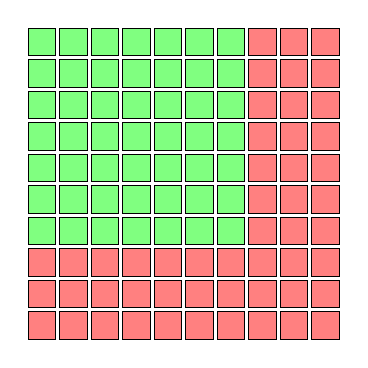
\begin{tikzpicture}[shorten >=1pt,->,draw=black!50, node distance=\layersep]
\tikzstyle{every pin edge}=[<-,shorten <=1pt]
\tikzstyle{neuron}=[rectangle, draw=black, fill=black!25, minimum size=10pt, inner sep=0pt]
\tikzstyle{input neuron}=[neuron, fill=green!50];
\tikzstyle{output neuron}=[neuron, fill=red!50];
\tikzstyle{hidden neuron}=[neuron, fill=blue!50];
\tikzstyle{annot} = [text width=4em, text centered]

% Draw the input layer nodes
\tikzmath{
    \scalenn = 0.4;
}

\foreach \x in {1,...,10}
    \foreach \y in {1,...,10}
        \ifthenelse {\x < 8 \AND \y < 8}
        {
            \node[input neuron] (I-\x-\y) at (\x * \scalenn,-\y * \scalenn) {};
        }
        {% else
            \node[output neuron] (I-\x-\y) at (\x * \scalenn,-\y * \scalenn) {};
        };

\end{tikzpicture}
% End of code
\end{document}
